\begin{frame}
	\myheading{Module 8.7 : Adding Noise to the inputs}
\end{frame}

\begin{frame}
	\vspace{4em}
	\begin{overlayarea}{\textwidth}{\textheight}
		\begin{block}{Other forms of regularization}
			\begin{itemize}
				\item $l_2$ regularization
				\item Dataset augmentation
				\item Parameter Sharing and tying
				\item \textcolor<2->{red}{Adding Noise to the inputs }
				\item Adding Noise to the outputs 
				\item Early stopping
				\item Ensemble methods
				\item Dropout
			\end{itemize}
		\end{block}
	\end{overlayarea}
\end{frame}
			

\begin{frame}
	\begin{columns}
		\column{0.3\textwidth}
							

		\begin{overlayarea}{\textheight}{\textwidth}
			\tikzstyle{input_neuron}=[circle,draw=red!50,fill=red!10,thick,minimum size=6mm]
\tikzstyle{hidden_neuron}=[circle,draw=blue!50,fill=cyan!10,thick,minimum size=6mm]
\tikzstyle{output_neuron}=[circle,draw=green!50,fill=green!10,thick,minimum size=6mm]
						
\tikzstyle{input}=[circle,draw=black!50,fill=black!20,thick,minimum size=6mm]
						
\begin{center}
	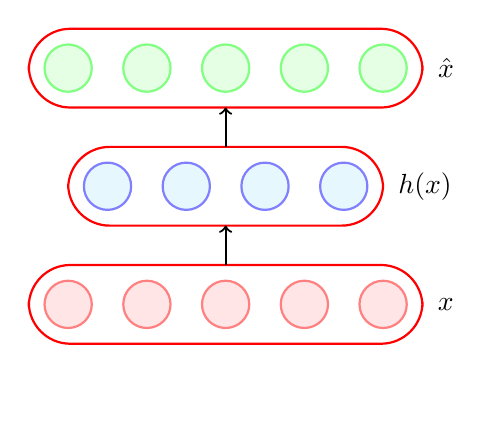
\begin{tikzpicture}
									
		\node (input0) at (6.5,3.5){};
		\node (input1) at (7.5,3.5){};
		\node (input2) at (8.5,3.5){};
		\node (input3) at (9.5,3.5){};
		\node (input4) at (10.5,3.5){};
		\node [input_neuron] (neuron01) at (6.5,4.5) {};
		\node [input_neuron] (neuron02) at (7.5,4.5){};
		\node [input_neuron] (neuron03) at (8.5,4.5) {};
		\node [input_neuron] (neuron04) at (9.5,4.5) {};
		\node [input_neuron] (neuron05) at (10.5,4.5) {};
		\node [hidden_neuron] (neuron51) at (7,6) {} ;
		\node [hidden_neuron] (neuron52) at (8,6)  {};
		\node [hidden_neuron] (neuron53) at (9,6)  {};
		\node [hidden_neuron] (neuron54) at (10,6)  {};
									
		\node [output_neuron] (neuron11) at (6.5,7.5)  {};
		\node [output_neuron] (neuron12) at (7.5,7.5)  {};
		\node [output_neuron] (neuron13) at (8.5,7.5)  {};
		\node [output_neuron] (neuron14) at (9.5,7.5)  {};
		\node [output_neuron] (neuron15) at (10.5,7.5)  {};
									
		\node[text width=0.01cm] at (11.2,4.5) {$x$};
		\node[text width=0.01cm] at (10.7,6) {$h(x)$};
		\node[] at (11.3,7.5) {$\hat{x} $};
		%\node[] at (12.5,7.5) {\footnotesize{$\hat{x}$}};
		\draw[red!100,thick,solid,rounded corners=15pt] (6,4) rectangle (11,5);
		\draw[red!100,thick,solid,rounded corners=15pt] (6.5,5.5) rectangle (10.5,6.5);
		\draw[red!100,thick,solid,rounded corners=15pt] (6,7) rectangle (11,8);
		\draw[thick,->] (8.5,5) -- (8.5,5.5);
		\draw[thick,->] (8.5,6.5) -- (8.5,7);
	\end{tikzpicture}
\end{center}
		\end{overlayarea}
							
		\column{0.5\textwidth}
							
		\begin{overlayarea}{\textwidth}{\textheight}
			\begin{itemize}
				\justifying
				\item<2-> We saw this in Autoencoder
				\item<3-> We can show that for a simple input output neural network, adding Gaussian noise to the input is equivalent to weight decay ($L_2$ regularisation)
				\item<4-> Can be viewed as data augmentation
			\end{itemize}
									
		\end{overlayarea}
							
	\end{columns}
\end{frame}
% %% page 3
			
			
\begin{frame}
	\Fontvi
	% \lipsum[1]
	\begin{columns}

		\column{0.35\textwidth}
		\vspace{2em}
		\hspace{2em}
		\begin{overlayarea}{\textwidth}{\textheight}
			
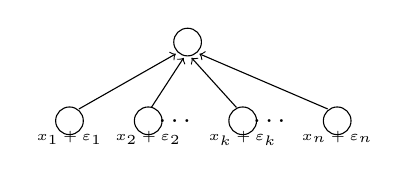
\begin{tikzpicture}
	\begin{scope}[every node/.style={sloped,allow upside down}]
		\draw (1.5,3) circle (0.5em);
		\draw (0,2) circle (0.5em)
		node[below=0.15] {\tiny $x_1 + \varepsilon_1$};
		\draw (1,2) circle (0.5em)
		node[below=0.15] {\tiny $x_2 + \varepsilon_2$}
		node[right=0.19] {\dots};
		\draw (2.2,2) circle (0.5em)
		node[below=0.15] {\tiny $x_k + \varepsilon_k$}
		node[right=0.19] {\dots};
		\draw (3.4,2) circle (0.5em) node[below=0.15] {\tiny $x_n + \varepsilon_n$};
		\draw[->] (0.12,2.15) -- (1.35,2.85);
		\draw[->] (1.04,2.17) -- (1.45,2.8);
		\draw[->] (2.12,2.17) -- (1.55,2.8);
		\draw[->] (3.28,2.15) -- (1.65,2.85);
	\end{scope}
\end{tikzpicture}
														
			\[
				\varepsilon \sim \mathcal{N}(0,\,\sigma^{2})    
			\] 
			\vspace{-1em}
			\begin{align*}
				\onslide<2->{\widetilde{x_i} & = x_i + \varepsilon_i                                     \\}
				\onslide<3->{\widehat{y}     & = \sum_{i=1}^{n}w_i x_i                                   \\}
				\onslide<4->{\widetilde{y}   & = \sum_{i=1}^{n}w_i \widetilde{x_i}                       \\}
				\onslide<5->{                & = \sum_{i=1}^{n}w_i x_i + \sum_{i=1}^{n}w_i \varepsilon_i \\}
				\onslide<6->{                & = \widehat{y} + \sum_{i=1}^{n}w_i \varepsilon_i  }        
			\end{align*}
		\end{overlayarea}
													
		\column{0.7\textwidth}
		\vspace{1em}
		\begin{overlayarea}{\textwidth}{\textheight}
			\onslide<7->{\hspace{2em}
				We are interested in $E[(\widetilde{y} - y)^2]$}
			\begin{align*}
				\onslide<8->{E\left[(\widetilde{y} - y)^2\right] & = E\left[\Big(\widehat{y} + \sum_{i=1}^{n}w_i \varepsilon_i - y \Big)^2\right] \\}
				\onslide<9->{                                    & = E\left[\left(  \Big(\widehat{y} - y \Big)+ \Big(\sum_{i=1}^{n}w_i \varepsilon_i \Big) \right)^2\right] \\}
				\onslide<10->{                                   & = E\left[(\widehat{y} - y)^2\right] + E\left[2(\widehat{y}-y) \sum_{i=1}^{n}w_i \varepsilon_i\right] + E\left[ \Big( \sum_{i=1}^{n}w_i \varepsilon_i \Big)^2\right] \\}
				\onslide<11->{                                   & = E\left[(\widehat{y} - y)^2\right] + 0 + E\left[\sum_{i=1}^{n}w_i^2 \varepsilon_i^2\right] \\
				                                                 & \text{($\because  \varepsilon_i$ is independent of $\varepsilon_j$ and $\varepsilon_i$ is independent of ($\widehat{y}$-$y$) )} \\}
				\onslide<12->{                                   & = (E\left[(\widehat{y} - y)^2\right] + \highlight{\sigma^2\sum_{i=1}^{n}w_i^2} \hspace{1em} \text{(same as }L_2 \text{ norm penalty)}}
			\end{align*}
		\end{overlayarea}
	\end{columns}
\end{frame}
